\documentclass[letterpaper,twocolumn,10pt]{article}
\usepackage{usenix-2020-09}

% to be able to draw some self-contained figs
\usepackage{tikz}
\usepackage{amsmath}

% inlined bib file
\usepackage{filecontents}

%-------------------------------------------------------------------------------
\begin{document}
%-------------------------------------------------------------------------------

%don't want date printed
\date{}

% make title bold and 14 pt font (Latex default is non-bold, 16 pt)
\title{\Large \bf Implementing a Secure Microservice Architecture:\\
  NGINX \& Kubernetes Deployment}

%for single author (just remove % characters)
\author{
{\rm Orchestration: Alexander Moomaw}\\
Eastern Washington University
\and
{\rm Services: Andree Ramirez}\\
Eastern Washington University
\and
{\rm Logging: Brendan Hopkins}\\
Eastern Washington University
\and
{\rm Frontend: Beighlor Martinez}\\
Eastern Washington University
\and
{\rm Defense: Cameron Olivier}\\
Eastern Washington University
\and
{\rm Services: Dillon Pikulik}\\
Eastern Washington University
\and
{\rm Project Management: Chelsea Edwards}\\
Eastern Washington University
}
% copy the following lines to add more authors
% \and
% {\rm Name}\\
%Name Institution
 % end author

\maketitle
%-------------------------------------------------------------------------------
\begin{abstract}
%-------------------------------------------------------------------------------
This paper presents a secure and scalable deployment architecture for web server environments using Kubernetes. 
The deployment incorporates a proxy and web application firewall for enhanced security and modular design. 
Additionally, we introduce our solution to logging and IP banning mechanisms to monitor and restrict unauthorized access. 
Our approach ensures high availability, load balancing, and robust defense against threats, offering a comprehensive framework for modern web applications.
\end{abstract}

%-------------------------------------------------------------------------------
\section{Introduction}
%-------------------------------------------------------------------------------
Ensuring the security and scalability of web server environments is a challenge in modern digital infrastructure. 
As cyber threats become more advanced, it's crucial to implement solutions that protect against unauthorized access 
while also maintaining high availability and performance. 

To address these challenges, we propose a comprehensive deployment architecture by first utilizing Kubernetes, an open-source platform designed for automating deployment, scaling, 
and management of containerized applications. With this platform, we ensure high-availability to prospective users and a modular
environment to build and scale upon as we please. 

To enhance our microservice architecture, we introduced an additional abstraction layer using an NGINX proxy hosted locally on the server. 
This proxy server fetches content from our Kubernetes load balancer, serving as a gateway between our internal services and external communications. 
To mitigate potential threats, we integrated ModSecurity, a well-known web application firewall (WAF), into our proxy. 
ModSecurity monitors and blocks common exploitation methods by referencing a comprehensive rule list that addresses the OWASP Top Ten vulnerabilities.

We realize that exploiting our endpoint services isn't the only attack vector within our environment. 
To address this, we implemented host-level logging to monitor network traffic and identify IP addresses not communicating via SSH or HTTP. 
Additionally, we applied an automated process to block malicious IP addresses, enhancing our overall security posture.



%-------------------------------------------------------------------------------
\section{Orchestration}
%-------------------------------------------------------------------------------
The ultimate challenge of any deployment life cycle is tying all ideas into a single, nicely wrapped package. This is the goal of orchestration.
To implement, or \textit{orchestrate} a deployment such as this, we designed a multi-tiered architectural diagram (Figure~\ref{fig:architecture})
that outlines how every building block in our environment fits together to form a finalized representation of a working project. 

% Add the figure
\begin{figure}[h]
    \centering
    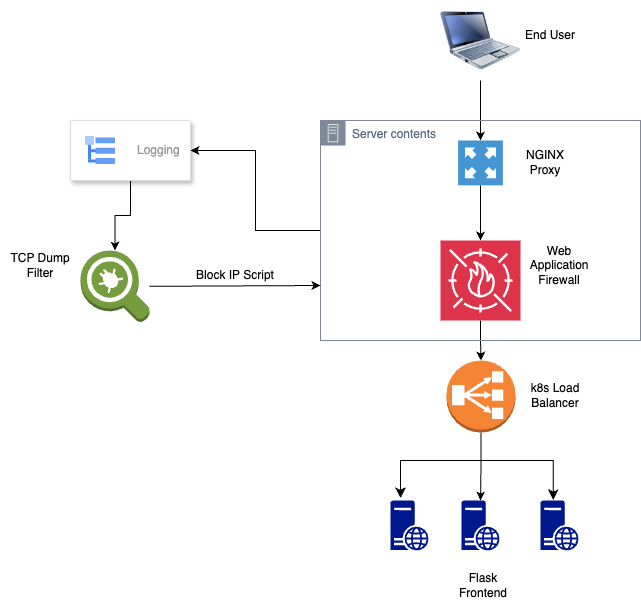
\includegraphics[width=\columnwidth]{resources/diagram.png} 
    \caption{Multi-tiered architectural diagram.}
    \label{fig:architecture}
\end{figure}

To host our content, we utilized Kubernetes. This method first involved integrating a docker image that was specifically designed to host content created by our frontend developers. We then created service and deployment YAML files to control multiple containers behind a load balancer. 

Once we had a functional cluster of orchestrated containers, the next goal was to make our load balancer not the first point of contact between external users and our internal environment. 
This involved integrating an NGINX reverse proxy ~\cite{nginx} on our host machine to facilitate communication without exposing our services directly to the internet. 

To setup an NGINX reverse proxy, we had to install the service then modify the global configuration file in the \texttt{/etc/nginx/conf.d/} directory to specifically mediate communications between external users and our internal load balancer ~\cite{hostinger_nginx_proxy}. The specifics for this step is
very convoluted, essentially we had to define server and location blocks with a \texttt{proxy pass} flag to enable the proxy feature of NGINX.

To tie our scalable, secure environment together on the orchestration end, we installed a web application firewall (WAF) on our reverse proxy to inspect requests being sent to the load balancer ~\cite{linode_modsecurity}. The requests
will be meticulously cross-referenced against a series of rule lists specifically designed to catch exploits matching the OWASP Top Ten vulnerabilities. If a exploit request is detected, the WAF will drop the request and return
a HTTP 403 status code to the threat actor.


%-------------------------------------------------------------------------------
\section{Logging and IP Gathering}


To enhance the security of our web server environment, we implemented a robust mechanism for gathering and logging IP addresses. This approach involves capturing IP addresses attempting 
to access our server on ports other than 22 (SSH) and 80 (HTTP) and maintaining comprehensive logs for further analysis. The IP gathering mechanism is designed to identify unauthorized access 
attempts by capturing IP addresses that try to connect to non-standard ports. This is achieved through a script that utilizes tcpdump to monitor network traffic and filter out unwanted connections. 
The captured IP addresses are stored in a cumulative list, which can be used to block malicious IPs via IP tables. In addition to gathering IP addresses, we implemented an hourly logging mechanism to 
maintain detailed records of network activity. This involves running a script that logs all IP traffic, excluding ports 22 and 80, and saves the logs with timestamps. These logs provide valuable data 
for analyzing traffic patterns and identifying potential security threats. To ensure the effectiveness of our IP gathering and logging mechanisms, the captured IP addresses and logs are periodically 
reviewed. This verification process involves accessing the log files to confirm that the security measures are functioning as intended and to identify any anomalies in network traffic.

%-------------------------------------------------------------------------------
\section{Defense}

We have established a comprehensive security protocol to monitor and block unauthorized access attempts to our web server. This involves capturing IP addresses attempting to access our server on ports other than 22 (SSH) and 80 (HTTP) and maintaining comprehensive logs for further analysis.

The process begins by clearing the log file \texttt{/var/log/honeypot/block_ip.log} to ensure new entries are recorded clearly. The script then checks for the existence of a cumulative IP list file at \texttt{/var/log/honeypot/ip_list_all.txt}, which contains IP addresses flagged for suspicious activity. If this list exists, the script reads each IP address and adds a \texttt{DROP} rule to \texttt{iptables}, effectively blocking incoming traffic from these addresses. The success or failure of each attempt to block an IP address is logged with a timestamp in the \texttt{block_ip.log} file. If the cumulative IP list is not found, an error message is logged and the script exits.

By employing this method, we aim to enhance our ability to detect and respond to potential security threats effectively. The combination of real-time IP address gathering, systematic logging, and automated blocking helps ensure that our web server environment remains secure and resilient against unauthorized access attempts.

%-------------------------------------------------------------------------------
\section{Threat Model}

The 'Weather and Jokes' web application employs Kubernetes and NGINX within its architecture to provide defenses against several cybersecurity threats. 
We are specifically defending against unauthorized access, SQL injections, Cross-Site Scripting (XSS), session hijacking, and Denial of Service (DoS) attacks. 
In contemplating the perceived capabilities of potential attackers, we recognize that they are likely to possess a high degree of technical sophistication, equipped with the skills necessary to exploit vulnerabilities typical of web applications. 
These attackers might use reconnaissance tools to gain information, and advanced techniques for SQL injections, craft XSS attacks, and leverage automated tools to execute DoS attacks.

To counter these threats, our application utilizes a load balancer within the Kubernetes environment to effectively manage traffic volumes that could potentially lead to DoS attacks. 
This load balancer helps distribute incoming traffic evenly across available servers, preventing any single server from becoming overwhelmed. We sanitize user input, protecting against XSS, and logging the attempts they made so we understand more of our attackers attacks and motives.
Additionally, NGINX, configured as a reverse proxy, is important in safeguarding against unauthorized access and filtering out malicious requests. It acts as a gatekeeper, routing all incoming traffic through its server and using ModSecurity-a web application firewall(Talked more about later)—to identify and block threats identified from patterns typical in SQL injections and XSS. 
Moreover, NGINX enhances the security of user sessions by managing encrypted connections, a crucial feature for preventing session hijacking. 
These encrypted channels ensure that session tokens, critical for maintaining user session integrity, are not intercepted or tampered with by unauthorized parties.
Through the strategic implementation of Kubernetes and NGINX, our application is well-prepared to defend against a wide spectrum of cybersecurity threats.

%-------------------------------------------------------------------------------
\section{Frontend Design}

\section{Frontend}
Our Website is called ‘Weather and Jokes’, and includes four pages: 'Home', 'Contact', 'FTP Manual', and 'Login'. The Home page runs two services, ‘Get a Joke’ and ‘Weather Checking’. The Contact page lists each of our team members and their roles within the group. The FTP Manual page gives instructions to our team members on how to use FTP. The FTP Manual page is meant to be a distraction for threat actors and is not fundamental to the actual Website, but rather a ploy to try and catch attackers attempting to use FTP. The final page, Login, takes in user input and redirects back to the log-in page. The log-in page never actually connects to any backend service, this page is used to try and catch potential threat actors attempting to use attacks such as SQL Injections.

%-------------------------------------------------------------------------------

%-------------------------------------------------------------------------------
\section{Services}

We have 2 services, both run in \verb+flask_example.py+ file and are presented on the \verb+index.html+ page. One of our services is utilizing a weather \verb+API+. This \verb+API+ has the weather in different geo locations around the world. We use this \verb+API+ to find the weather of a website’s geo location. The user has a \verb+textbox+ on the \verb+index.html+ page that they can enter the websites \verb+URL+. After they enter the \verb+URL+ they can hit the \verb+button+ to get the weather. We ask for user input of a website's \verb+URL+ and output the current weather of that website. This is done by taking the \verb+URL+ and running \verb+gethostbyname+ to get the IP address of that \verb+URL+. Now after we get the IP address, we run a \verb+whois+ command on the IP address. This command will give us a lot of information on the IP address, but we parse out the physical address associated with the IP. After the physical address is parsed and formatted for the \verb+API+ we call \verb+(https://geocoding.geo.census.gov/) API+ and get returned the \verb+X,Y+ geo coordinates of that address ~\cite{GeoLocationAPI}. Now that we have geo coordinates we can send those to the weather \verb+API+. The weather \verb+API+ is at \verb+https://api.weather.gov/points/+, where we input the coordinates at the end of the \verb+URL+ to get back the weather ~\cite{WeahterAPI}. After we send the coordinates, we receive the weather of that location, which is the location of the initially given website. All of these command are automated in the \verb+flask_example.py+ file. I chose to implement this service because I have done it in the past and had very well-documented files that aided in quick implementation. This in return aided the rest of the team by speeding up the process of deployment. This service also is very large and can be used for about every website, this could keep the attacks busy, possibly giving information away about themselves.

Another \verb+API+ service that was utilized was the\verb+ /joke+ route in the \verb+Flask+ application serving a random dad joke to the user. When accessed, the function \verb+joke()+ is executed, which sets the \verb+API URL https://icanhazdadjoke.com/+ and defines a \verb+cURL+ command to request a joke in plain text format ~\cite{DadJokesAPI}. The \verb+subprocess.run+ function runs this command and captures the output, which contains the joke. Finally,  \verb+result.stdout+ is returned, sending the joke back to the user's browser. Additionally, there is a clickable button in \verb+index.html+ that allows users to retrieve a joke, providing a simple and interactive way to display a random dad joke. The reason this service was chosen was to have clickable and interactable features on the websites so that targets on the website are encouraged to click more and give potential information.




%-------------------------------------------------------------------------------

%-------------------------------------------------------------------------------
\section{Evaluation Methodology}
%-------------------------------------------------------------------------------
Here you may want your evaluation methodology...

\label{sec:figs}
%-------------------------------------------------------------------------------


%---------------------------
\begin{figure}
\begin{center}
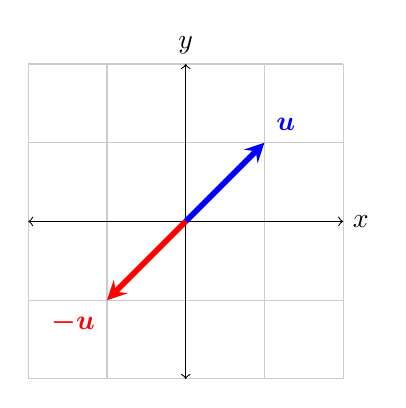
\begin{tikzpicture}
  \draw[thin,gray!40] (-2,-2) grid (2,2);
  \draw[<->] (-2,0)--(2,0) node[right]{$x$};
  \draw[<->] (0,-2)--(0,2) node[above]{$y$};
  \draw[line width=2pt,blue,-stealth](0,0)--(1,1)
        node[anchor=south west]{$\boldsymbol{u}$};
  \draw[line width=2pt,red,-stealth](0,0)--(-1,-1)
        node[anchor=north east]{$\boldsymbol{-u}$};
\end{tikzpicture}
\end{center}
\caption{\label{fig:vectors} Text size inside figure should be as big as
  caption's text. Text size inside figure should be as big as
  caption's text. Text size inside figure should be as big as
  caption's text. Text size inside figure should be as big as
  caption's text. Text size inside figure should be as big as
  caption's text. }
\end{figure}
%% %---------------------------


Here's a typical reference to a floating figure:
Figure~\ref{fig:vectors}. Floats should usually be placed where latex
wants then. Figure\ref{fig:vectors} is centered, and has a caption
that instructs you to make sure that the size of the text within the
figures that you use is as big as (or bigger than) the size of the
text in the caption of the figures. Please do. Really.

In our case, we've explicitly drawn the figure inlined in latex, to
allow this tex file to cleanly compile. But usually, your figures will
reside in some file.pdf, and you'd include them in your document
with, say, \textbackslash{}includegraphics.

Lists are sometimes quite handy. If you want to itemize things, feel
free:

\begin{description}
  
\item[fread] a function that reads from a \texttt{stream} into the
  array \texttt{ptr} at most \texttt{nobj} objects of size
  \texttt{size}, returning returns the number of objects read.

\item[Fred] a person's name, e.g., there once was a dude named Fred
  who separated usenix.sty from this file to allow for easy
  inclusion.
\end{description}

\noindent
The noindent at the start of this paragraph in its tex version makes
it clear that it's a continuation of the preceding paragraph, as
opposed to a new paragraph in its own right.


\subsection{LaTeX-ing Your TeX File}
%-----------------------------------

People often use \texttt{pdflatex} these days for creating pdf-s from
tex files via the shell. And \texttt{bibtex}, of course. Works for us.




%-------------------------------------------------------------------------------
\section{Results}
%-------------------------------------------------------------------------------
  The first test run was an SQL Injection on the Login page, using the expression " admin' OR '1'='1' -- " in the user input with " password"  in the password input. Normal behavior would just redirect the page back to itself, however because it detected an SQL Injection the page was forwarded to a 403 Forbidden page, and the suspicious activity was logged, with  the time of attempted access, the attempted username, the attempted password, and the IP address of the attacker. The next attack we used was an SQL injection in the password input where user input was " user " , and password input was " wrongpassword' OR 'a'='a " again we got the same results as the first attempt, a it forwarded the client to a 403 forbidden page was and the suspicious activity was logged. 

  The second test we ran was cross site scripting or XSS, so in normal behavior the pages would redirect normally, so 10.102.68.91/about to 10.102.68.91/home, however in testing we added an XSS script at the end of the url to test the behavior of our webpages. The command we used was http://10.102.67.91/about=</script><script>alert(0)</script>, an XSS script that would thrown an alert on the webpage. However our defense worked as intended redirecting to a 403 forbidden page and did not create the XSS alert as the attacker intended. The suspicious activity was logged and given to our security team so they could block the IP address of the potential attacker. This 403 error actually gets thrown any time there is a reference using </script>. The normal activity for the webpage is to redirect to a url not found, for example if you enter 10.102.68.91/about=user it will redirect to URL not found, so any XSS or added script will be blocked by our firewall. We made sure to test each of our pages, home, about, manual, and login, and each page passed as intended.

    The third test we ran was for command injection we again used on our login page. In normal behavior a successful login attempt would redirect back to the login page. The attack we tested command injection is a type of attack that takes advantage of a program using a operating system call, for example if our program ran ping and displayed results of the ping, an attacker would be able to input ' 8.8.8.8;ls ' to display information about whats inside their current directory. The ' ;ls ' is the attack and 8.8.8.8 would be the normal input. So in our test we used the username input ' user;ls ' and password as ' password ', the firewall successully blocked this attack and redirected the page to a 403 forbidden page and logged the suspicious activity, alerting our monitoring team and indicating another successful test. 



%-------------------------------------------------------------------------------
\section{Conclusion}
%-------------------------------------------------------------------------------
Our web server security solution deploys and scales with Kubernetes, supported by an NGINX proxy and ModSecurity for increased protection. Host-level logging and automated IP blocking further strengthen security. Using a multi-tiered architecture and Kubernetes hosting, we integrate and orchestrate these components seamlessly. An NGINX reverse proxy ensures secure communication while a web application firewall examines and blocks known vulnerabilities.

To enhance security, we implemented a mechanism that logs IP addresses trying to access non-standard ports, with hourly logs for network activity monitoring. We utilize Docker to run our website 'Weather and Jokes' with Ubuntu and Flask, providing isolated defensive features. The website includes four pages: Home, Contact, FTP Manual (honeypot), and Login (trap for attackers).

Two services in the flask_example.py file fetch weather and dad jokes using APIs. The weather service converts URLs to IP addresses, retrieves physical addresses, and obtains weather based on geographical coordinates. The joke service offers an interactive feature for users.

In order to evaluate our infrastructure, we conduct simulated attacks, including SQL injection, cross-site scripting (XSS), and command injection, which our web application firewall successfully detects and blocks, as confirmed by HTTP 403 responses.

\bibliographystyle{plain}
\bibliography{refs}

%%%%%%%%%%%%%%%%%%%%%%%%%%%%%%%%%%%%%%%%%%%%%%%%%%%%%%%%%%%%%%%%%%%%%%%%%%%%%%%%
\end{document}
%%%%%%%%%%%%%%%%%%%%%%%%%%%%%%%%%%%%%%%%%%%%%%%%%%%%%%%%%%%%%%%%%%%%%%%%%%%%%%%%

%%  LocalWords:  endnotes includegraphics fread ptr nobj noindent
%%  LocalWords:  pdflatex acks
